\documentclass[a4paper]{extarticle}
\usepackage[utf8]{inputenc}
\usepackage[a4paper, margin=1in]{geometry}

\usepackage{amssymb}
\usepackage{amsmath}
\usepackage{enumitem}
\usepackage{tcolorbox}
\usepackage{fancyhdr}
\usepackage{graphicx}
\usepackage{float}

\setlength{\parindent}{0em}
\setlength{\parskip}{0.4em}

\definecolor{theoremblue}{RGB}{1, 73, 124}
\definecolor{corollaryblue}{RGB}{70, 143, 175}
\definecolor{exampleblue}{RGB}{137, 194, 217}

\newtcolorbox{tbox}{colback=theoremblue!20,colframe=theoremblue,
boxrule=0pt,arc=0pt,boxsep=2pt,left=2pt,right=2pt,leftrule=2pt}

\newtcolorbox{cbox}{colback=corollaryblue!20,colframe=corollaryblue,
boxrule=0pt,arc=0pt,boxsep=2pt,left=2pt,right=2pt,leftrule=2pt}

\newtcolorbox{ebox}{colback=exampleblue!20,colframe=exampleblue,
boxrule=0pt,arc=0pt,boxsep=2pt,left=2pt,right=2pt,leftrule=2pt}

\title{WuS - Lecture Notes Week 1}
\author{Ruben Schenk, ruben.schenk@inf.ethz.ch}
\date{\today}

\pagestyle{fancy}
\fancyhf{}
\rhead{ruben.schenk@inf.ethz.ch}
\rfoot{Page \thepage}
\lhead{WuS - Lecture Notes Week 1}

\begin{document}

\maketitle
\newpage


\section{Introduction}

\subsection{Percolation Theory}

\subsubsection{Overview}

In physics and mathematics, \textbf{percolation theory} describes the behavior of clustered components in random networks. The common intuition is movement and filtering of fluids through porous materials, for example, filtration of water through soil and permeable rocks. In a network, let each node be a cell through which a fluid-like substance may transit to other cells. A network, i.e. a grid, then is a sponge-like substance and percolation is the determination of whether a substance introduced at one cell will reach the other side of the network (or grid).

\subsubsection{Percolation in a Box}

Imagine a box (or grid) with vertices \(V = \{-n,...,n\}^2\) and edges \(E = \{e_1,...,e_N\}\). We introduce parameter \(p\), with \(0 \leq p \leq 1\). \(p\) denotes the probability that an edge \(e\) is \textit{open} (\(X_e = 1\)). In other words, an edge \(e\) is \textit{closed} (\(X_e = 0\)) with probability \(1-p\). The corresponding model could look something like this:

\begin{figure}[H]
    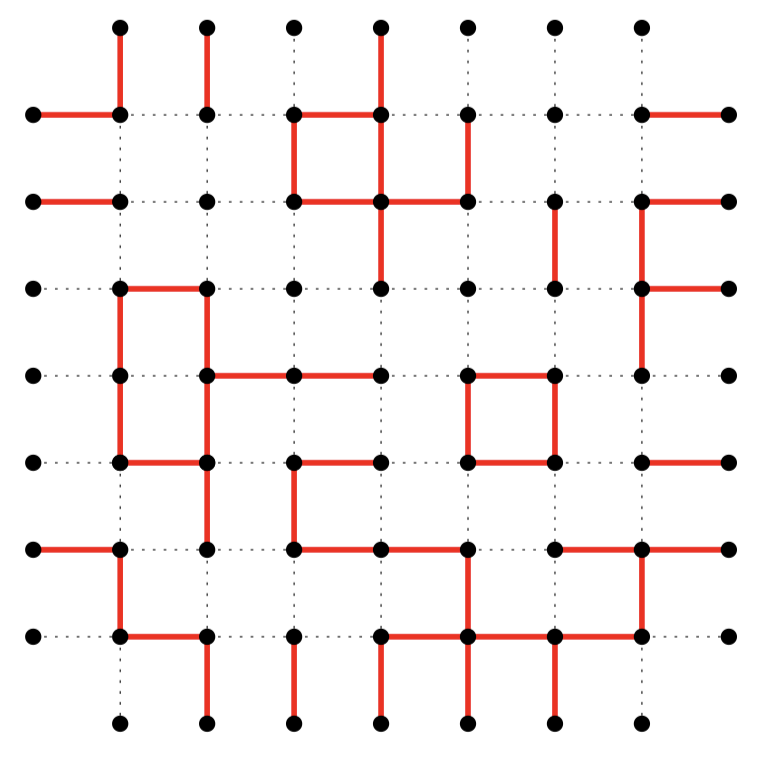
\includegraphics[width=6cm]{../images/WuS_Fig1-1}
    \centering
\end{figure}

\textit{Note:} If an edge is colored red, it means that it's open.

We denote an \textbf{open path} as a path consisting of open edges. A \textbf{cluster} is the connected component of \((V, \, \{e : X_e = 1\})\). The following figure shows an example of a cluster (marked in blue):

\begin{figure}[H]
    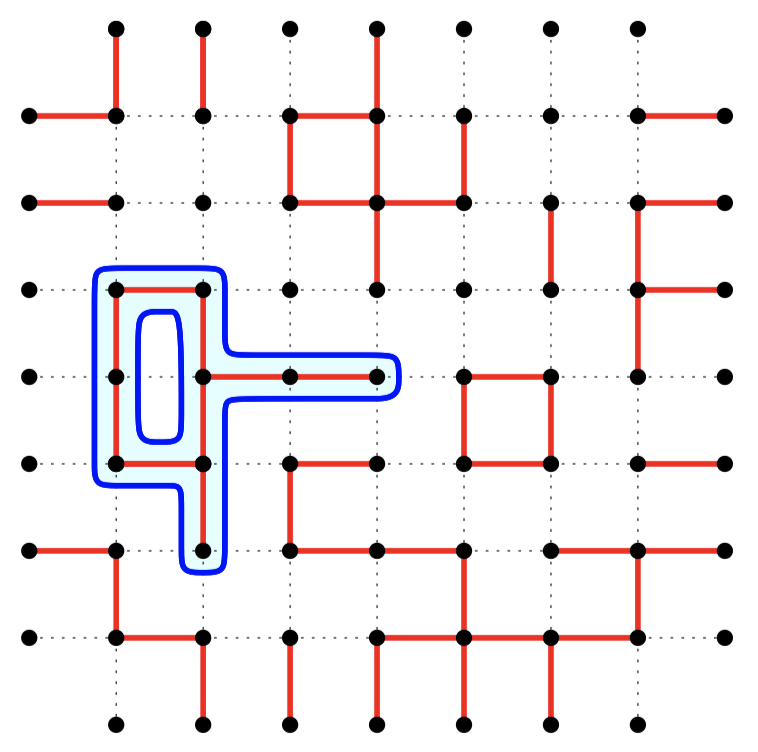
\includegraphics[width=6cm]{../images/WuS_Fig1-2}
    \centering
\end{figure}

\begin{tbox}
    \textbf{Theorem [Kesten, 1980]:} For the percolation with parameter \(p\) we have:
    \[
        \lim_{n \to \infty} \mathbb{P} [\bullet] = \begin{cases}
            0, \quad &\text{if } p < \frac{1}{2}, \\ 1, \quad &\text{if } p > \frac{1}{2}.
        \end{cases}
    \]
    where \(\mathbb{P}[\bullet]\) denotes the probability that there exists an open path from the top to the bottom in an \(n \times n\) box.
    Similarly, for the percolation with parameter \(p\) we have:
    \[
        \mathbb{P}[\exists \text{ an infinite cluster}] = \begin{cases}
            0, \quad &\text{if } p < \frac{1}{2}, \\ 1, \quad &\text{if } p > \frac{1}{2}.
        \end{cases}
    \]
\end{tbox}

\subsection{Introduction to Probability}

\textbf{Probability} is a mathematical language describing systems involving randomness. Probabilities are used for:

\begin{itemize}
    \item \textit{Describe random experiments} in the real world, such as coin flips, dice rolling, etc.
    \item \textit{Express uncertainty.} For example, when a machine performs a measurement, the value is rarely exact. One may use probability theory in this context by saying that the value obtained is equal to the real value plus some small random error.
    \item \textit{Decision-making.} Probability theory can be used to describe a system when only part of the information is known.
    \item \textit{Randomized algorithms} in computer science. Sometimes, it is more efficient to add some randomness to perform an algorithm.
    \item \textit{Simplify complex systems.} Examples include water molecules in water, cars on the highway, etc.
\end{itemize}

The \textbf{goal} of probability theory is to establish general theorems which describe the behavior of multiple random experiments. Example:

\begin{tbox}
    \textbf{Theorem [Law of large numbers]:}
    \[
        X_i = \begin{cases}
            0, \quad &i^{th} \text{ throw is head,} \\ 1, \quad &i^{th} \text{ throw is number.}
        \end{cases}  
    \]
    It holds, that:
    \[
        \lim_{n \to \infty} \frac{X_1 + \cdots + X_n}{n} = \frac{1}{2}.
    \]
\end{tbox}

\section{Mathematical Framework}

\subsection{Probability Space}

\subsubsection{Sample Space}

Assume we want to model a random experiment. The first mathematical object needed is the set of all possible outcomes of the experiment, denoted by \(\Omega\).

The set \(\Omega\) is called the \textbf{sample space.} An element \(\omega \in \Omega\) is called an \textbf{outcome} (or \textit{elementary experiment}).

\begin{ebox}
    \textbf{Example:} If we throw a die, we have the following sample space:
    \[
        \Omega = \{1, \, 2, \, 3, \, 4, \, 5, \, 6\}  
    \]
\end{ebox}

\subsubsection{Events}

Previously, the set of \textbf{events} was always \(\mathcal{P}(\Omega)\). In this class, we will work with more general sets of events \(\mathcal{F} \subset \mathcal{P}(\Omega)\), called sigma algebras.

\textbf{Definition:} A \textbf{sigma-algebra} is a subset \(\mathcal{F} \subset \mathcal{P}(\Omega)\) satisfying the following properties:

\begin{enumerate}
    \item \(\Omega \in \mathcal{F}\)
    \item \(A \in \mathcal{F} \implies A^C \in \mathcal{F}\)
    \item \(A_1, A_2,... \in \mathcal{F} \implies \bigcup_{i = 1}^{\infty} A_i \in \mathcal{F}\)
\end{enumerate}

\begin{ebox}
    \textbf{Example:} Following are some (non-) examples of sigma-algebras for \(\Omega = \{1, \, 2, \, 3, \, 4, \, 5, \, 6\}\):

    \begin{itemize}
        \item \(\mathcal{F} = \{\emptyset, \, \{1, \, 2, \, 3, \, 4, \, 5, \, 6\}\}\) is a sigma-algebra.
        \item \(\mathcal{F} = \{\emptyset, \, \{1, \, 2\}, \, \{3, \, 4, \, 5, \, 6\}, \, \{1, \, 2, \, 3, \, 4, \, 5, \, 6\}\}\) is a sigma-algebra.
        \item \(\mathcal{F} = \{\{1, \, 2, \, 3, \, 4, \, 5, \, 6\}\}\) is not a sigma-algebra because \(P2\) is not satisfied.
        \item \(\mathcal{F} = \{\emptyset, \, \{1, \, 2, \, 3\}, \, \{4, \, 5, \, 6\}, \, \{1\}, \, \{2, \, 3, \, 4, \, 5, \, 6\}, \, \Omega\}\) is not a sigma-algebra because \(P3\) is not satisfied.
    \end{itemize}
\end{ebox}

\subsubsection{Probability Measure}

\textbf{Definition:} Let \(\Omega\) be a sample space, let \(\mathcal{F}\) be a sigma-algebra. A \textbf{probability measure} on \((\Omega, \, \mathcal{F})\) is a map

\begin{align*}
    \mathbb{P} : &\mathcal{F} \to [0, \, 1] \\
    &A \to \mathbb{P}[A]
\end{align*}

that satisfies the following two properties:

\begin{itemize}
    \item \textbf{P1.} \(\mathbb{P}[\Omega] = 1\).
    \item \textbf{P2. (countable additivity)} \(\mathbb{P}[A] = \sum_{i = 1}^{\infty} \mathbb{P}[A_i]\) if \(A = \bigcup_{i = 1}^{\infty} A_i\) (\textit{disjoint union}).
\end{itemize}

\subsubsection{Notion of Probability Space}

\textbf{Definition:} Let \(\Omega\) be a sample space, \(\mathcal{F}\) a sigma-algebra, and \(\mathbb{P}\) a probability measure. The triple \((\Omega, \, \mathcal{F}, \, \mathbb{P})\) is called a \textbf{probability space.}

\end{document}